

%%%%%%%%%%%%%%%%%%%%%%%%%%%%%%%%%%%%%%%%%%%%%%%%%%
\subsection{Polarization and Stokes Parameters}


Polarized light is light in which the electric field has a preferred orientation. For linearly polarized light, the electric field oscillates along a fixed direction perpendicular to the direction in which the light propagates \citep{RybickiLightman} (see Figure \ref{fig: LinearPol}). Polarization information from interferometers (such as ALMA) is represented by the Stokes visibilities from cross-correlations between antennas in the array \citep{HullDebias}. The Stokes parameter $I$ is the total intensity of the emission. \SQ measures the difference in intensity between the North-South and East-West components. \SU measures the difference between the components at 45$^\circ$ and 135$^\circ$ relative to the North-South axis. This coordinate system is shown in Figure \ref{fig: LinearPol}. The \SQ and $U$ parameters together provide information about the strength and orientation of the linear polarization. Circular polarization adds another Stokes parameter ($V$), however, ALMA is not well calibrated to observe circular polarization. \question{cite something for this?}




\begin{figure}[htbp]
  \centering
  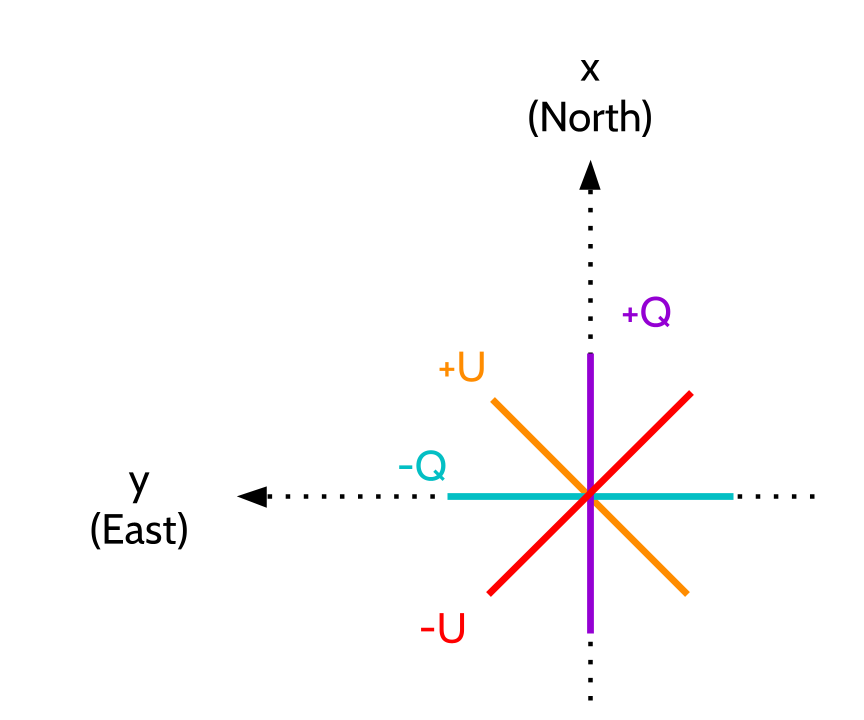
\includegraphics[width=0.5\textwidth]{WRITEUP_AND_IMAGES/IMAGES/WRITEUP/Intro/StokesQU.png}
  \caption{Coordinate system for the Stokes parameters $Q$ and $U$.}
  \label{fig: LinearPol}
\end{figure}


%%%%%%%%%%%%%%%%%%%%%%%%%%%%%%%%%%%%%%%%%%%%%%%%%%

\subsection{Polarization Mechanisms}
\label{sec: intro_polarization_mechanisms}
% \note{In Chapter \ref{sec: c4_polarization_maps} I refer to this section for a reasoning on why a circular pattern can be from radiative alignment, or some other unknown reason} "This is consistent with the pattern expected from radiative alignment (or some other mechanism, Chapter \ref{sec: intro_polarization_mechanisms}), shown in Figure \ref{fig: kataoka_polarization_morphologies}(b). "


The polarization angle from the emission is used to construct polarization vectors(Chapter \ref{sec: chap4_polarization_vectors}), revealing the polarization morphology, or pattern. Different polarization mechanisms produce different morphologies, and each can help constrain different physical properties of the disk \citep{Stephens_2019}. Because multiple mechanisms can produce polarized emission at (sub)millimetre wavelengths, it is a challenge to disentangle and identify the dominant polarization mechanism \citep{Kataoka_2017}. The following paragraphs explore several potential mechanisms and their morphologies, but this is not a complete list. Examples of the polarization morphologies produced by different mechanisms are shown in  Figure \ref{fig: kataoka_polarization_morphologies}. 



% Polarization observations of polarized emission from dust grains in disks at (sub)millimetre wavelengths provide insight into dust grain growth in protostellar disks \citep{Harrison2024}.  



% ------------------------------------------------
\begin{figure}[htbp]
  \centering
  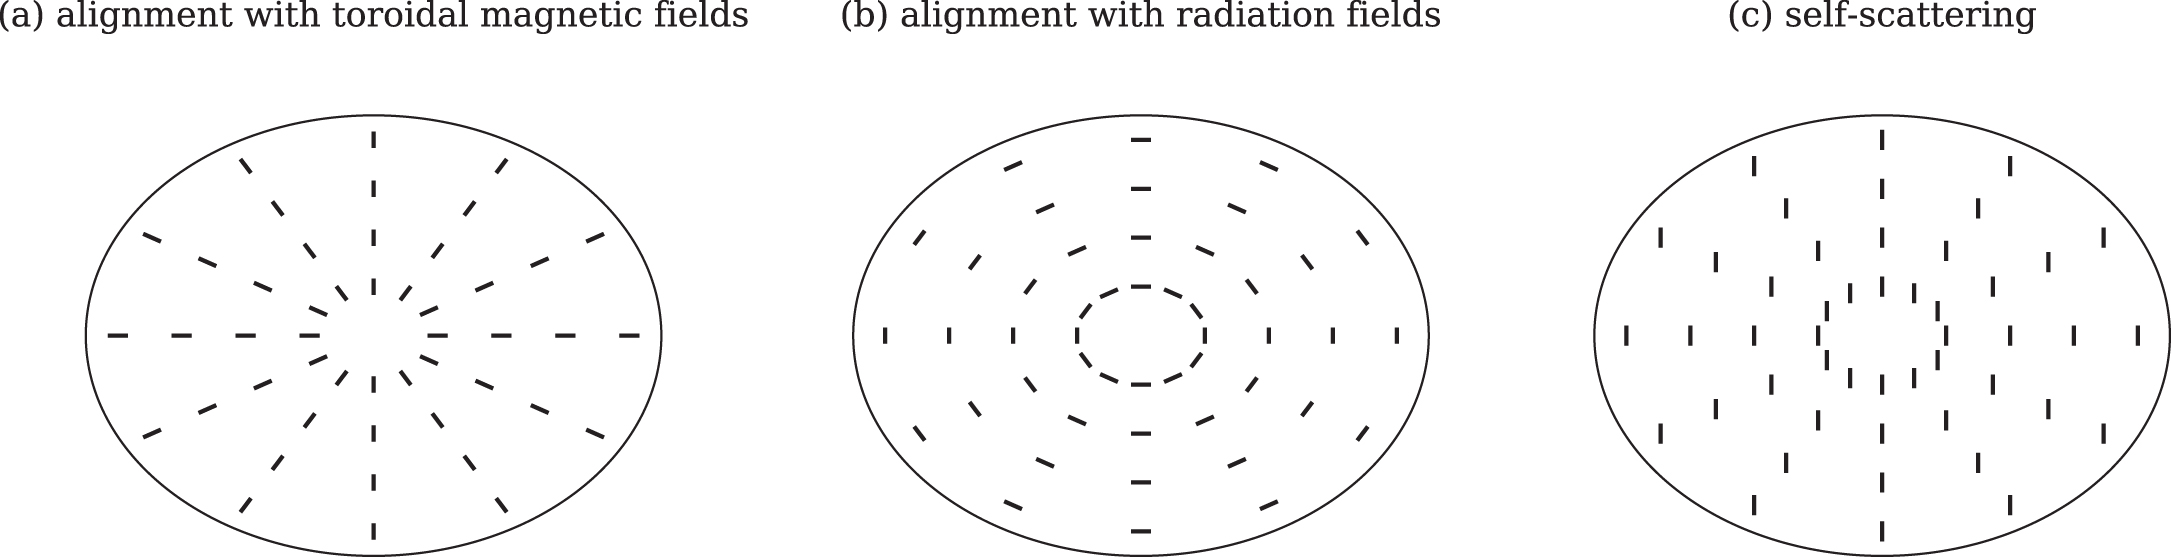
\includegraphics[width=1.0\textwidth]{WRITEUP_AND_IMAGES/IMAGES/WRITEUP/NOTMINE/apjlaa7e33f3_hr.jpg}
  \caption{Schematic of three polarization morphologies and a potential mechanism causing them. The image is from \cite{Kataoka_2017}. \permission{ask permission to use} }
  \label{fig: kataoka_polarization_morphologies}
\end{figure}
% ------------------------------------------------




%%%%%%%%%%%%%%%%%%%%%%%%%%%%%%%%%%%%%%%%%%%%%%%%%%


\question{Is this a good way to differentiate the three paragraphs?} 

\textbf{Magnetic Grain Alignment.} Magnetic grain alignment is produced when the short axis of non-spherical dust grains aligns parallel to the magnetic field direction via radiative torques  \citep{Stephens_2019, Harrison2024}. The polarization morphology produced by magnetic grain alignment is expected to be toroidal \citep{Stephens_2017}, which can be seen in Figure \ref{fig: kataoka_polarization_morphologies}(a). Polarized dust emission is known to trace the magnetic field direction in the ISM, molecular clouds and potentially in the outer regions of disks \citep{Stephens_2019}. Despite magnetic grain alignment being the expected mechanism for producing polarization in disks, it is often not observed. Instead, the pattern observed in most disks is generally better explained by other mechanisms  \citep{Harrison2024}. 






%%%%%%%%%%%%%%%%%%%%%%%%%%%%%%%%%%%%%%%%%%%%%%%%%%





%%%%%%%%%%%%%%%%%%%%%%%%%%%%%%%%%%%%%%%%%%%%%%%%%%
%%%%%%%%%%%%%%%%%%%%%%%%%%%%%%%%%%%%%%%%%%%%%%%%%%

\textbf{Radiative Grain Alignment.} Radiative alignment occurs when non-spherical grains align with the radiation field, with the long axis of the grains being perpendicular to the radiation field (k-RAT alignment) \citep{Stephens_2017}. This produces a polarization morphology that is azimuthal, meaning the polarization vectors follow a circular pattern about the centre of the disk, as shown in Figure \ref{fig: kataoka_polarization_morphologies}(b). However, an azimuthal polarization morphology can also be produced by other mechanisms. For example, mechanical alignment can occur when grains align with their long axis in the streaming direction \citep{Stephens_2019}, or aerodynamic alignment can occur when gas and dust orbit the central star at different speeds. Therefore, the exact mechanism responsible for this morphology cannot be determined based only on the morphology, and is not a main goal of the project. In this thesis, the azimuthal morphology is a description of the pattern rather than evidence for a single specific polarization mechanism. 


% \quoted{Multiple mechanisms could
% theoretically produce this polarized emission, including radiation anisotropy (Tazaki et al. 2017), aerodynamic alignment due to gas–dust interactions (Gold 1952; Yang et al. 2019), . }\cite{Harrison2024}



% \quoted{Several mechanisms have been proposed for grain alignment, including alignment to the magnetic field or radiation anisotropy through radiative alignment torques (RATs; Tazaki et al. 2017) }\cite{Harrison2024}


% \quoted{Several mechanisms have been proposed for grain alignment, including mechanical alignment (Gold 1952; Kataoka et al. 2019; Yang et al. 2019).}\cite{Harrison2024}



%%%%%%%%%%%%%%%%%%%%%%%%%%%%%%%%%%%%%%%%%%%%%%%%%%







%%%%%%%%%%%%%%%%%%%%%%%%%%%%%%%%%%%%%%%%%%%%%%%%%%


\textbf{Dust Self-Scattering.} Dust self-scattering occurs when thermal emission from dust grains is scattered by other dust grains in the disk, producing polarized emission. This mechanism is expected to produce a polarization morphology that is roughly parallel to the disk minor axis \citep{Kataoka_2017}, as shown in Figure \ref{fig: kataoka_polarization_morphologies}(c). The efficiency of dust self-scattering polarization is highly dependent on the maximum grain size (see Chapter \ref{sec: c5_P_and_w_vs_a}), so it is useful for constraining the maximum dust grain size \citep{Harrison2024}. This sensitivity to grain size makes dust self-scattering a useful mechanism to focus on in this project. 









% \quoted{In addition to the
% dust grain size, the disk inclination, optical depth, and dust
% scale height can all affect the level of polarization from
% scattering (e.g., Yang et al. 2017; Ohashi and Kataoka 2019;
% Brunngräber and Wolf 2020).}\cite{Harrison2024}


%  % ------------------------------------------------
% \begin{figure*}[h]
%   \centering
%   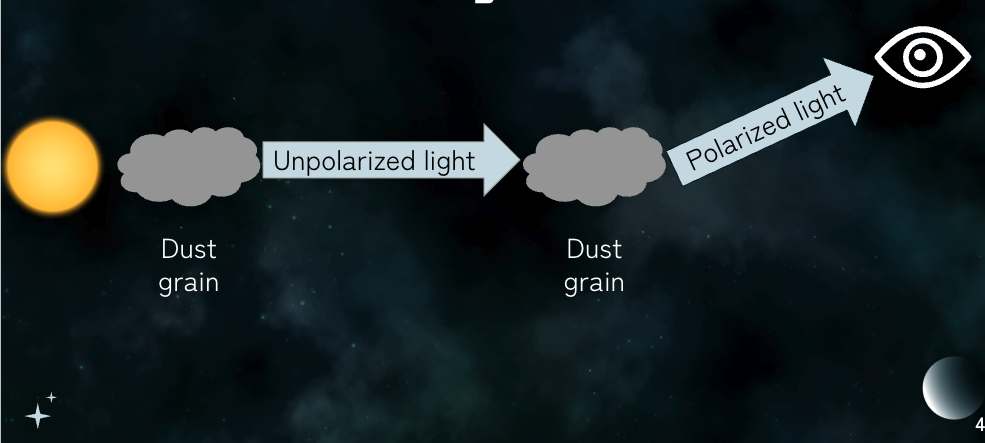
\includegraphics[width=0.8\textwidth]{WRITEUP_AND_IMAGES/IMAGES/SLIDESHOW_SCREENSHOT/dust_self_scattering_schematic.png}
%   \caption{\add{caption}}
%   \label{fig: dust-self-scattering-schematic}
% \end{figure*}
% % ------------------------------------------------


























